\documentclass[a4]{beamer}
\usepackage{amssymb}
\usepackage{graphicx}
\usepackage{subfigure}
\usepackage{newlfont}
\usepackage{amsmath,amsthm,amsfonts}
%\usepackage{beamerthemesplit}
\usepackage{pgf,pgfarrows,pgfnodes,pgfautomata,pgfheaps,pgfshade}
\usepackage{mathptmx}  % Font Family
\usepackage{helvet}   % Font Family
\usepackage{color}

\mode<presentation> {
 \usetheme{Default} % was Frankfurt
 \useinnertheme{rounded}
 \useoutertheme{infolines}
 \usefonttheme{serif}
 %\usecolortheme{wolverine}
% \usecolortheme{rose}
\usefonttheme{structurebold}
}

\setbeamercovered{dynamic}

\title[MA4413]{MA4413 Statistics for Computing \\ {\normalsize MA4413 Lecture 6A : Continuous Distributions}}
\author[Kevin O'Brien]{Kevin O'Brien \\ {\scriptsize kevin.obrien@ul.ie}}
\date{Autumn 2011}
\institute[Maths \& Stats]{Dept. of Mathematics \& Statistics, \\ University \textit{of} Limerick}

\renewcommand{\arraystretch}{1.5}


%------------------------------------------------------------------------%
\begin{document}
\frame{
\frametitle{Midterm Exam}
\begin{itemize}
\item 1300hr on Tuesday (Week 7)
\item Worth 15\% of overall mark for module.
\item The test is comprised of 15 short questions, or components of compound questions.
\item Topics:
\begin{itemize}
\item Basic Probability
\item The Binomial Distribution
\item The Poisson Distribution
\item The Normal Distribution
\end{itemize}
\item Revision lecture on Monday of Week 7.
\end{itemize}
}
%------------------------------------------------------------------------%
\begin{frame}
\large
\frametitle{Today's Class}
\begin{itemize}
\item Introduction to Continuous Random Variables
\item Probability Density Functions
\item Density Curves
\item Cumulative Distribution Functions
\item Exact Probabilities
\item The Complement Rule and Intervals
\item The Continuous Uniform Distribution
\item The Exponential Distribution

\end{itemize}
\end{frame}
%----------------------------------------------------------------------------------------------------%
\frame{
\frametitle{Continuous Random Variable}
A continuous random variable is one which takes an infinite number of possible values.\\ Continuous random variables are usually measurements. Examples include height, weight, the amount of sugar in an orange, the time required to run a mile.
\\
\bigskip
In this module, we will look at random variables from the following distributions
\begin{itemize}
\item Continuous uniform probability distribution
\item Exponential probability distribution
\item Normal probability distribution
\end{itemize}

Before this, we will look at some important concepts.
}

%----------------------------------------------------------------------------------------------------%
\begin{frame}
\frametitle{Functions and Definite integrals}
\begin{itemize}
\item Integration is not part of the syllabus, and it is assumed that students have are not familiar with how to compute definite integrals.
\item However,  it is useful to know what the purpose of definite integrals are, because we will be using the results derived from definite integrals. \item It is assumed that students are familiar with functions.
\end{itemize}
\end{frame}
%----------------------------------------------------------------------------------------------------%
\begin{frame}
\frametitle{Functions}

\vspace{-0.5cm}

\begin{center}
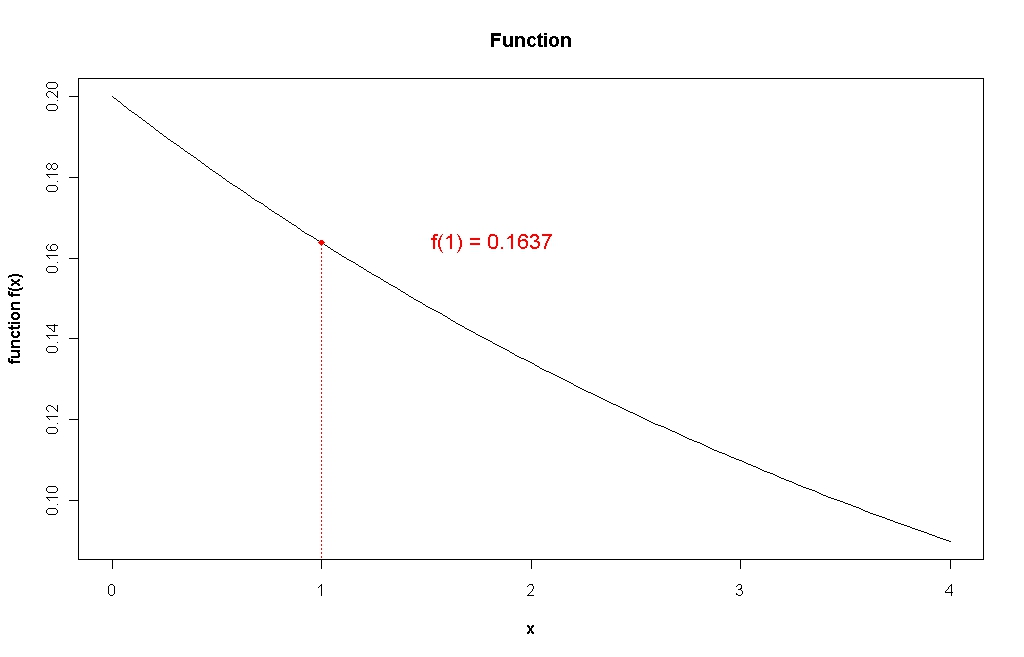
\includegraphics[scale=0.30]{6AFunction}

\end{center}

Some function $f(x)$ evaluated at $x=1$.
\end{frame}
%----------------------------------------------------------------------------------------------------%
\begin{frame}
\frametitle{Definite Integral}

\vspace{-0.5cm}
\begin{center}
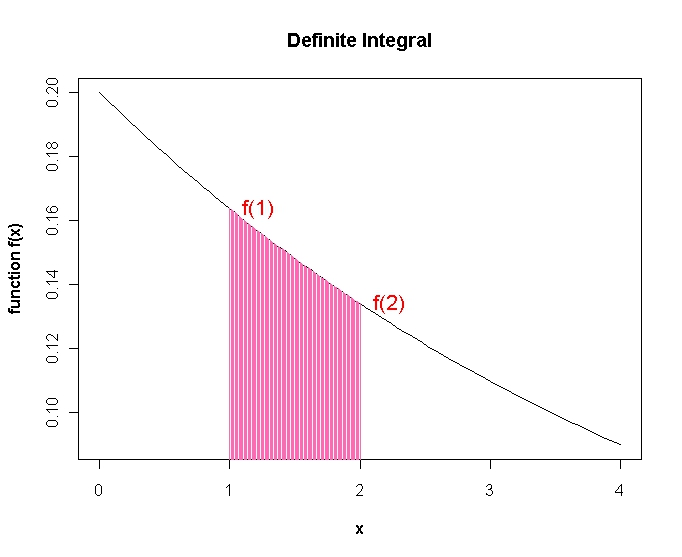
\includegraphics[scale=0.35]{6ADefiniteIntegral}
\end{center}
Definite integral of function is area under curve between X=1 and X=2.
\end{frame}
%----------------------------------------------------------------------------------------------------%
\begin{frame}
\frametitle{Definite Integral}
\begin{itemize}
\item Definite integrals are used to compute the ``area under curves".
\item Definite integrals are defined by a lower and upper limit.
\item The area under the curve between X=1 and  X=2 is depicted in the previous slide.
\item By computing the definite integral, we are able to determine a value for this area.
\item Probability can be represented as an area under a curve.
\end{itemize}
\end{frame}

%----------------------------------------------------------------------------------------------------%
\frame{

\frametitle{Probability Density Function}
\begin{itemize}
\item
In probability theory, a \textbf{\emph{probability density function}} (pdf) (or ``density" for short ) of a continuous random variable is a function that describes the relative likelihood for this random variable to occur at a given point.

\item The pdf for a continuous random variable $X$ is often denoted $f_X(x)$

\item The probability density function can be integrated to obtain the probability that the random variable takes a value in a given interval.

\item The probability for the random variable to fall within a particular interval is given by the integral of this variable's density over the region.

\item The probability density function is non-negative everywhere, and its integral over the entire space is equal to one.
\end{itemize}
}

%----------------------------------------------------------------------------------------------------%
\frame{
\frametitle{Probability Mass Function}

\begin{itemize}
\item The equivalent of a pdf for discrete distributions is the \textbf{\emph{probability mass function }} (pmf).
\item The probability mass function is often the primary means of defining a discrete probability distribution.
\item We have encountered p.m.f.s before; for the binomial and Poisson distribution.
\item A probability mass function (pmf) is a function that gives the probability that a discrete random variable is exactly equal to some value i.e. $P(X =1)$.
\item We generally don't require integration for this calculations.
\end{itemize}
}

%----------------------------------------------------------------------------------------------------%

\begin{frame}

\frametitle{Density Curves}


\begin{itemize}
\item A plot of the pdf is referred to as a `\textbf{\emph{density curve}}'.
\item A density curve that is always on or above the horizontal axis and has total area underneath equal to one.
\item Area under the curve in a range of values indicates the proportion of values in that range.
\item Density curves come in a variety of shapes, but the normal distribution's bell-shaped densities are the commonly used.
\item Remember the density is only an approximation, but it simplifies analysis and is generally accurate enough for practical use.
\end{itemize}
\end{frame}
%----------------------------------------------------------------------------------------------------%
\frame{
\frametitle{The Cumulative Distribution Function }
\begin{itemize}
\item The \textbf{\emph{cumulative distribution function}} (CDF), (or just distribution function), describes the probability that a continuous random variable X with a given probability distribution will be found at a value less than or equal to x.\\

\[ F_X(x) = P(X \leq x) \]

\item Intuitively, it is the ``area so far" function of the probability distribution.
\end{itemize}

}
%----------------------------------------------------------------------------------------------------%
\begin{frame}
\frametitle{Cumulative Distribution Function}

\vspace{-0.5cm}
\begin{center}
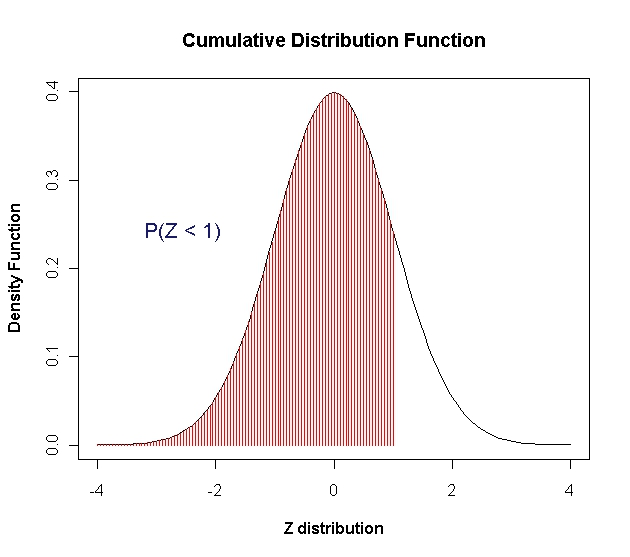
\includegraphics[scale=0.35]{6ACDF}

\end{center}
Cumulative Distribution Function $P(Z \leq 1)$.
\end{frame}
%------------------------------------------------------------------%
\frame{
\frametitle{Exact Probability}
\large
\alert{Remarks:} This is for continuous distributions only.
\begin{itemize}
\item The probability that a continuous random variable will take an exact value is infinitely small.
We will usually treat it as if it was zero.
\item
When we write probabilities for continuous random variables in mathematical notation, we often retain the equality component (i.e. the "...or equal to..").\\
For example, we would write expressions $P(X \leq 2)$ or $P(X \geq 5)$.
\item
Because the probability of an exact value is almost zero, these two expression are equivalent to $P(X < 2)$
or $P(X > 5)$. \item The complement of $P(X \geq k)$ can be written as $P(X \leq k)$.
\end{itemize}
}

%------------------------------------------------------------------%
\frame{
\frametitle{The Complement Rule}
\large

\begin{itemize}
\item When studying the normal distribution, we came across the \textbf{\emph{Complement rule}}.
\[ P(X \leq k ) = 1 - P(X \geq k) \] for some value $k$.
\item The complement rule applies to all continuous distributions, not just the normal distribution.
\item When studying the normal distribution, we also came across the \textbf{\emph{Symmetry rule}}.
\item This rule is specific to the standard normal distribution. It can not be used for other distributions.
\end{itemize}
}
%------------------------------------------------------------------%
\frame{
\frametitle{Intervals}
\large

\begin{itemize}
\item When computing the probability that some value lies within an interval $(L,U)$, we used the ``Too low/Too high" approach.

\item This approach can be used with all continuous probability distributions.
\end{itemize}
}



%---------------------------------------------------------------------------%
\frame{
\frametitle{Continuous Uniform Distribution}
A random variable X is called a continuous uniform random variable over the interval $(a,b)$ if it's probability density function is given by
\[ f_{X}(x) = { 1 \over b-a} \hspace{1cm} \mbox{ when } a \leq x \leq b \mbox{     (otherwise } f_X(x) = 0 ) \]
The corresponding cumulative density function is
\[ F_x(x) = { x-a \over b-a} \hspace{1cm} \mbox{ when } a \leq x \leq b\]
}
%----------------------------------------------------------------------------------------------------%
\begin{frame}
\frametitle{The Continuous Uniform Distribution}

\vspace{-0.5cm}

\begin{center}
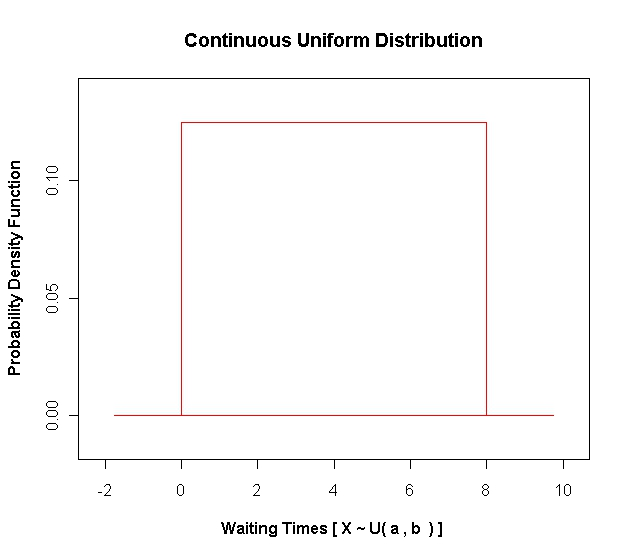
\includegraphics[scale=0.35]{6AUniform}

\end{center}
\end{frame}
%---------------------------------------------------------------------------%
\frame{
\frametitle{Continuous Uniform Distribution}
\begin{itemize}
\item The continuous distribution is very simple to understand and implement, and is commonly used in computer applications (e.g. computer simulation).
\item It is also known as the `Rectangle Distribution' for obvious reasons.
\item We specify the word ``continuous" so as to distinguish it from it's discrete equivalent: the discrete uniform distribution.
\item Remark; the dice distribution is a discrete distribution with lower and upper limits 1 and 6 respectively.
\end{itemize}
}

\frame{
\frametitle{Uniform DistributionParameters}


The continuous uniform distribution is characterized by the following parameters

\begin{itemize}
\item The lower limit $a$
\item The upper limit $b$
\item We denote a uniform random variable $X$ as $X \sim U(a,b)$
\end{itemize}

It is not possible to have an outcome that is lower than $a$ or larger than $b$.

\[ P(X < a) = P(X > b) = 0\]
}

%------------------------------------------------------------------------%
\frame{\frametitle{Interval Probability}

\begin{itemize}
\item We wish to compute the probability of an outcome being within a range of values.
\item We shall call this lower bound of this range $L$ and the upper bound $ U$.
\item Necessarily $L$ and $U$ must be possible outcomes.
\item The probability of $X$ being between $L$ and $U$ is denoted $P( L \leq X \leq U )$.

\[
P( L \leq X \leq U ) = { U - L \over b - a}
\]
\item (This equation is based on a definite integral).
\end{itemize}
}
%---------------------------------------------------------------------------------------------------------%
\frame{
\frametitle{Uniform Distribution: Cumulative Distribution}
\begin{itemize}

\item For any value ``c" between the minimum value a and the maximum
value $b$, we can say
\item $P(X \geq c)$ \[P(X \geq c) = {b-c \over b-a}\]
here $b$ is the upper bound while $c$ is the lower bound
\item $P(X \leq c)$ \[P(X \leq c) = {c-a \over b-a}\]
here $c$ is the upper bound while $a$ is the lower bound.
\end{itemize}
}

%-----------------------------------------------------------------------------%
\frame{
\frametitle{Uniform Distribution: Mean and Variance}
\begin{itemize}
\item The mean of the continuous uniform distribution, with parameters $a$ and $b$ is
\[ E(X) = {a+b \over 2}\]
\item The variance is computed as
\[ V(X) = {(b-a)^2 \over 12}\]
\end{itemize}
}
%------------------------------------------------------------------------%
\frame{
\frametitle{Uniform Distribution: Example}

\begin{itemize}
\item Suppose there is a platform in a subway station in a large large city. \item Subway trains arrive \textbf{every three minutes} at this platform. \item What is the shortest possible time a passenger would have to wait for a train?
\item What is the longest possible time a passenger will have to wait?
\end{itemize}

}


%------------------------------------------------------------------------%
\frame{
\frametitle{Uniform Distribution: Example}

\begin{itemize}
 \item What is the shortest possible time a passenger would have to wait for a train?
%\begin{itemize}
\item If the passenger arrives just before the doors close, then the waiting time is zero.
\[ a = 0 \mbox{ minutes } \]
\end{itemize}
}


%------------------------------------------------------------------------%
\frame{
\frametitle{Uniform Distribution: Example}

\begin{itemize}
\item What is the longest possible time a passenger will have to wait?
%\begin{itemize}
\item If the passenger arrives just after the doors close, and missing the train, then he or she will have to wait the full three minutes for the next one.
\[ b = 3 \mbox{ minutes }  = 180 \mbox{ seconds}  \]
\end{itemize}
%\end{itemize}

}

%------------------------------------------------------------------------%
\frame{
\frametitle{Uniform Distribution: Example}

\begin{itemize}
\item What is the longest probability that he will have to wait longer than 2 minutes?
\[ P(X \geq 2)  = {3-2 \over 3-0} = {1/3} = 0.33333   \]
\end{itemize}
%\end{itemize}

}

%----------------------------------------------------------------------------------------------------%
\begin{frame}
\frametitle{The Continuous Uniform Distribution}

\vspace{-0.5cm}

\begin{center}
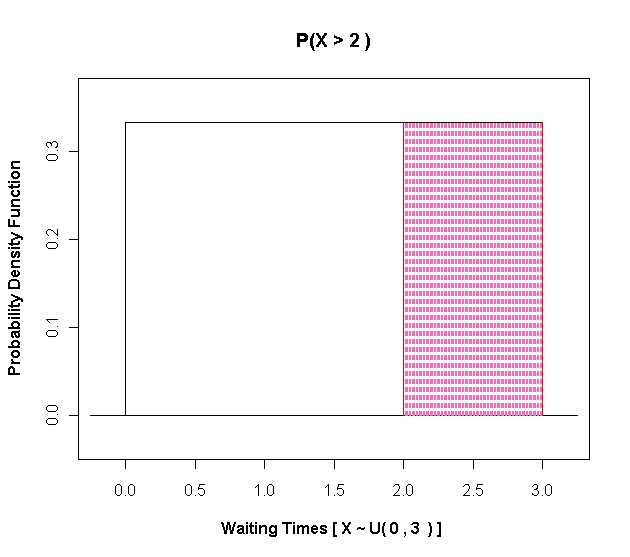
\includegraphics[scale=0.35]{6AUniform4}

\end{center}
\end{frame}
%------------------------------------------------------------------------%
\frame{
\frametitle{Uniform Distribution: Example}

\begin{itemize}
\item What is the longest probability that he will have to wait less than than 45 seconds (i.e. 0.75 minutes)?
\[ P(X \leq 0.75)  = {0.75 - 0 \over 3-0} = {0.75/3} = 0.250  \]
\end{itemize}
%\end{itemize}

}
%----------------------------------------------------------------------------------------------------%
\begin{frame}
\frametitle{The Continuous Uniform Distribution}

\vspace{-0.5cm}

\begin{center}
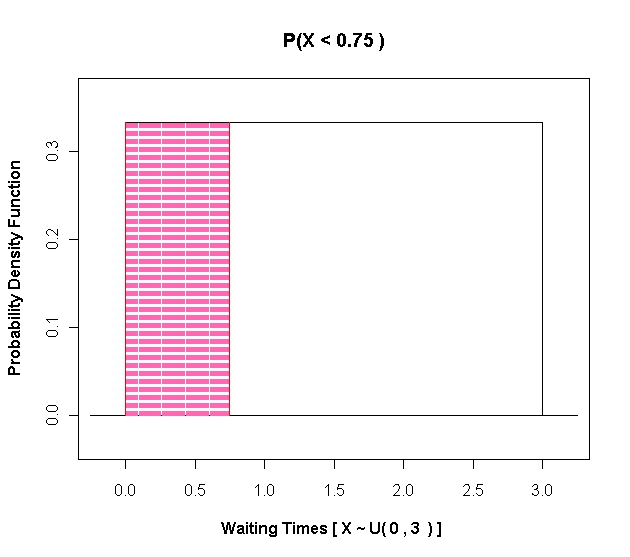
\includegraphics[scale=0.35]{6AUniform3}

\end{center}
\end{frame}
%------------------------------------------------------------------------%
\frame{
\frametitle{Uniform Distribution: Expected Value}

We are told that, for waiting times,  the lower limit $a$ is 0, and the upper limit $b$ is 3 minutes. \\ \bigskip The expected waiting time $\textrm{E}[X]$ is computed as follows
\vspace{0.1cm}
\[
\textrm{E}[X] = {b + a \over 2} =  {3 + 0  \over 2}  = 1.5 \mbox{ minutes }
\]

}
%------------------------------------------------------------------------%
\frame{\frametitle{Uniform Distribution: Variance}

The variance of the continuous uniform distribution, denoted $\textrm{V}[X]$,  is  computed using the following formula
\vspace{0.1cm}
\[
\textrm{V}[X] = {(b - a)^2 \over 12}
\]
\vspace{0.1cm}
For our previous example this is
\[
\textrm{V}[X] = {(3 - 0)^2 \over 12} =  {3^2 \over 12} = {9 \over 12} = 0.75
\]
}


%--------------------------------------------------------------------------------------%
\begin{frame}
\frametitle{The Exponential Distribution}
\begin{itemize}
\item The exponential distribution is a continuous probability distribution commonly used to model durations or ``lifetimes".
\item A lifetime could mean
\begin{itemize}
\large
\item the lifespan of a component
\item the time it takes to complete a task
\item the amount of time between two successive occurrences, such as withdrawals from a bank machine.
\end{itemize}
\item The average lifetime is denoted $E(X) = \mu$.
\item The variance of lifetimes is computed as $V(X) = \mu^2$
\end{itemize}
\end{frame}

%--------------------------------------------------------------------------------------%
\frame{
\frametitle{Important Formulae}
\Large
The probability that a lifetime $X$ will be less than a period of $k$ time units is given by
\[
P( X \leq k) = 1- e^{{-k \over \mu}}.
\]
Similarly, the probability that a lifetime $X$ will be greater than a period of $k$ time units is given by
\[
P( X \geq k) = e^{{-k \over \mu}}.
\]
}
%--------------------------------------------------------------------------------------%
\frame{
\frametitle{Sample Question}
\Large
In a large company computer network, there is an average of 40 log-ons to the network per hour.
\begin{enumerate}
\item[1] What is the average amount of time between log-ons?
\item[2] What is the probability that there will be no log-ons for at least 2.4 minutes
\item[3] What is the probability that the next log-on within 1 minutes of the last?
\item[4] What proportions of log-ons occur between 1 minutes and 2.4 minutes of the last log-on?
\end{enumerate}
}
%--------------------------------------------------------------%
\frame{
\frametitle{Solution (Part 1) }

\Large
\begin{itemize} \item What is the average amount of time between log-ons?

\item If there is 40 log-ons in 60 minutes, it is reasonable to think that someone logs on every 1.5 minutes.
\item Therefore $\mu = 1.5$
\end{itemize}

}
%--------------------------------------------------------------------------------------%
\frame{
\frametitle{Solution (Part 2) }
\Large

What is the probability that there will be no log-ons for at least 2.4 minutes?\\
\bigskip
From the formulae:
\[
P( X \geq k) = e^{{-k \over \mu}} .
\]
From the formulae:
\[
P( X \geq 2.4) = e^{{-2.4 \over 1.5}} = e^{-1.6} = 0.2018.
\]
}

%--------------------------------------------------------------------------------------%
\frame{
\frametitle{Solution (Part 3) }
\Large

What is the probability that the next log-on within 1 minutes of the last?\\
i.e. $P(X \leq 1)$
\bigskip
From the formulae:
\[
P( X \leq 1) = 1 - e^{{-1 \over 1.5}} = 1 -  e^{-0.6666}
\]

\[
P( X \leq 1) = 1 -  0.5135  = 0.4865
\]
}

%--------------------------------------------------------------------------------------%
\frame{
\frametitle{Solution (Part 4) }
\Large

What proportions of log-ons occur between 1 minutes and 2.4 minutes of the last log-on?\\
\bigskip
\begin{itemize}
\item \textbf{Too Low} $P(X \leq 1) = 0.4865$\\
\item \textbf{Too High} $P(X \geq 2.4) = 0.2018$\\
\item Probability of being inside interval $P(1 \leq X \leq 2.4) = 0.31152$.
\item $P(1 \leq X \leq 2.4) = 1- ( 0.4865 + 0.2018) = 0.3117$
\end{itemize}
}
\end{document}





\item What is the probability that the lifespan of the laptop will be at least
6 years?
\item What is the probability that the lifespan of the laptop will not exceed
4 years?
\item What is the probability of the lifespan being between 5 years and 6
years?


%----------------------------------------------------------------------------%
\frame{
\frametitle{The Exponential Distribution}
A continuous random variable having p.d.f. f(x), where:
$f(x) = \lambda x e ^{-\lambda x} $
is said to have an exponential distribution, with parameter $\lambda$.
The cumulative distribution is given by:
$F(x) = 1 - e^{\lambda x}$

Expectation and Variance
$E(X) = 1 / \lambda$\\
$V(X) = 1 / \lambda^2$\\
}

%----------------------------------------------------------------------------%
\frame{
\frametitle{Example}
Suppose that the service time for a customer at a fast-food outlet
has an exponential distribution with mean 3 minutes. What is the probability that a
customer waits more than 4 minutes?

\[ P(X  \leq 4) = 1 -  e^{-4/3} \]

\[ P(X  \leq 4) = e^{-4/3} = 0.2636 \]
}


%---------------------------------------------------------------------------------%
\begin{frame}
\frametitle{Exponential Distribution Lifetimes}
The average lifespan of a laptop is 5 years. You may assume that
the lifespan of computers follows an exponential probability
distribution. \begin{itemize}\item (3 marks) What is the
probability that the lifespan of the laptop will be at least 6
years? \item
What is the probability that the lifespan of the laptop will not
exceed 4 years? \item What is the probability of the
lifespan being between 5 years and 6 years?
\end{itemize}
Suppose the lifetime of a PC is exponentially distributed with
mean $\mu =5$
We should be told the average lifetime $\mu$.
\[
P( X \geq x_o) = e^{{-x_o \over \mu}}
\]
\end{frame}


\end{document}








